\documentclass{standalone}
\usepackage{graphicx}	
\usepackage{amssymb, amsmath}
\usepackage{color}

\usepackage{tikz}
\usetikzlibrary{intersections, backgrounds, math}
\usepackage{pgfmath}

\definecolor{light}{RGB}{220, 188, 188}
\definecolor{mid}{RGB}{185, 124, 124}
\definecolor{dark}{RGB}{143, 39, 39}
\definecolor{highlight}{RGB}{180, 31, 180}
\definecolor{light_teal}{RGB}{107, 142, 142}
\definecolor{mid_teal}{RGB}{72, 117, 117}
\definecolor{dark_teal}{RGB}{29, 79, 79}
\definecolor{gray10}{gray}{0.1}
\definecolor{gray20}{gray}{0.2}
\definecolor{gray30}{gray}{0.3}
\definecolor{gray40}{gray}{0.4}
\definecolor{gray60}{gray}{0.6}
\definecolor{gray70}{gray}{0.7}
\definecolor{gray80}{gray}{0.8}
\definecolor{gray90}{gray}{0.9}
\definecolor{gray95}{gray}{0.95}

\begin{document}

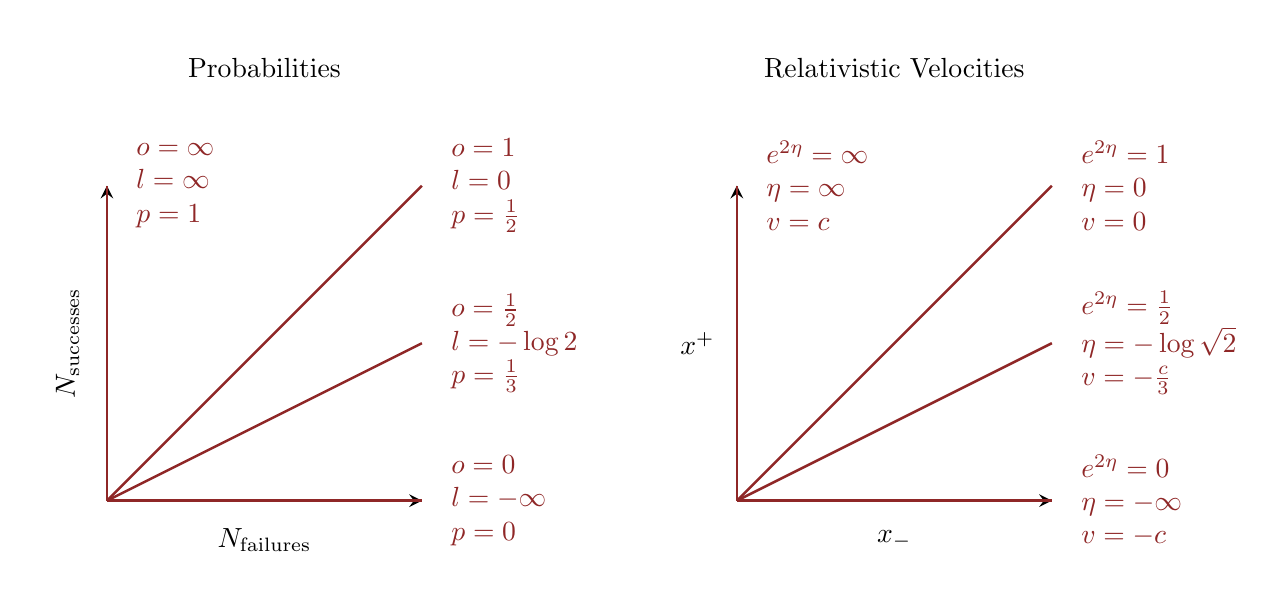
\begin{tikzpicture}[scale=1.0]
  \begin{scope}[shift={(0, 0)}]
    \draw[white] (-1, -1) rectangle (6.5, 6);

    \node at (2, 5.5) { Probabilities };
  
    \draw [->, >=stealth, line width=1] (0, 0) -- (4, 0);
    \node at (2, -0.5) { $N_{\text{failures}}$ };
  
    \draw [->, >=stealth, line width=1] (0, 0) -- (0, 4);
    \node[rotate=90] at (-0.5, 2) { $N_{\text{successes}}$ };
  
    \draw[dark, line width=0.9] (0, 0) -- (4, 4);
    \node[dark, align=left, anchor=west] at (4.25, 4) { $o = 1$\\$l = 0$\\$p = \frac{1}{2}$ };
  
    \draw[dark, line width=0.9] (0, 0) -- (4, 0);
    \node[dark, align=left, anchor=west] at (4.25, 0) { $o = 0$\\$l = -\infty$\\$p = 0$ };
  
    \draw[dark, line width=0.9] (0, 0) -- (0, 4);
    \node[dark, align=left, anchor=west] at (0.25, 4) { $o = \infty$\\$l = \infty$\\$p = 1$ };
  
    \draw[dark, line width=0.9] (0, 0) -- (4, 2);
    \node[dark, align=left, anchor=west] at (4.25, 2) { $o = \frac{1}{2}$\\$l = - \log 2$\\$p = \frac{1}{3}$ };
  \end{scope}

  \begin{scope}[shift={(8, 0)}]
    \draw[white] (-1, -1) rectangle (6.5, 6);

    \node at (2, 5.5) { Relativistic Velocities };
  
    \draw [->, >=stealth, line width=1] (0, 0) -- (4, 0);
    \node at (2, -0.5) { $x_{-}$ };
  
    \draw [->, >=stealth, line width=1] (0, 0) -- (0, 4);
    \node at (-0.5, 2) { $x^{+}$ };
  
    \draw[dark, line width=0.9] (0, 0) -- (4, 4);
    \node[dark, align=left, anchor=west] at (4.25, 4) 
      { $e^{2 \eta} = 1$\\$\eta = 0$\\$v = 0$ };
  
    \draw[dark, line width=0.9] (0, 0) -- (4, 0);
    \node[dark, align=left, anchor=west] at (4.25, 0)
      { $e^{2 \eta} = 0$\\$\eta = -\infty$\\$v = -c$ };
  
    \draw[dark, line width=0.9] (0, 0) -- (0, 4);
    \node[dark, align=left, anchor=west] at (0.25, 4)
      { $e^{2 \eta} = \infty$\\$\eta = \infty$\\$v = c$ };
  
    \draw[dark, line width=0.9] (0, 0) -- (4, 2);
    \node[dark, align=left, anchor=west] at (4.25, 2)
      { $e^{2 \eta} = \frac{1}{2}$\\$\eta = - \log \sqrt{2}$\\$v = -\frac{c}{3}$ };
  \end{scope}
\end{tikzpicture}

\end{document}  